%!TEX root = ../abgabe.tex

\section{Einführung}

Written by Dima

In diesem Kapitel werden notwendige Kenntnisse zum Verständnis dieser Arbeit  eingeführt. Zunächst werden die wesentlichen Begriffe „mobiler Kontext“ und „Mobilgerät“ erklärt. Anschließend  werden verschiedene Eingabe- und Ausgabemöglichkeiten in den Mobilgeräten vorgestellt und auf die Schwierigkeiten, mit denen ein Designer konfrontieren muss, eingegangen.
\subsection{Was ist mobiler Kontext} % (fold)
\label{sub:was_ist_mobiler_kontext}
Bevor wir über das Design für mobilen Kontext sprechen, müssen wir zuerst klar stellen, was ein "mobiler Kontext" bedeutet. In dem Buch "The Mobile Frontier: A Guide for Designing Mobile Experiences“ beschreibt die Autorin, Rachel Hinman, ein Experiment, das im 2006 von einer Forschungsgruppe durchgeführt wurde und den Begriff des mobilen Kontext definiert. Eine Gruppe von Versuchspersonen wurde gebeten, die Orte zu fotografieren, an denen sie ihre Mobilgeräte nutzen. Die Forscher hofften, dass nach einer Analyse dieser Aufnahmen sie die grundlegenden Prinzipien des mobilen Kontexts bestimmen können. Nach einer Woche erhielten sie eine hohe Anzahl an Fotos von vollkommen unterschiedlichen Orten und Situationen.[7]

 \begin{figure}[h]
 \centering
 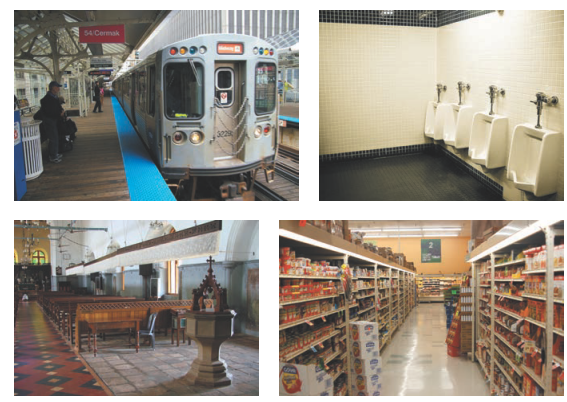
\includegraphics[height=0.25\textheight]{img/studie.png}
 \caption{Pictures of the mobile context from a dairy study on mobile Internet access[7]}
\end{figure}

Die Fotos wurden unterwegs auf der Straße, im Supermarkt, im Bus oder im Zug, sowie auch an unerwarteten Orten, wie in einem Restaurant, im Schlafzimmer und sogar in einer Kirche geschossen. Selbst nach einer langen Sortierung, Kategorisierung und Analyse konnten sie dennoch kein Muster für den "mobilen Kontext" erkennen. Daraufhin kamen sie zu der Definition "Mobile context = anywhere and everywhere", was auf Deutsch übersetzt bedeutet: „mobiler Kontext“ ist immer und überall. Meiner Meinung nach ist das eine gute Bezeichnung dafür. Da im Vergleich zu der Interaktion mit dem herkömmlichen PC, geschieht die Interaktion im mobilen Kontext mitten im Leben des Benutzers. Verschiedene Mobilgeräte wie z.B. Smartphones  begleiten den Nutzer von morgens bis abends, oft bis ins Bett. Und die Aufgabe des Designers ist, das zu berücksichtigen und den Nutzern gute Bedienbarkeit anzubieten.

% subsubsection was_ist_mobiler_kontext (end)
\subsection{Mobilgeräte} % (fold)
\label{sub:mobile_ger_te}
Es gibt keine einheitliche und spezifizierte Definition von dem Begriff „Mobilgerät“. Man kann das Mobilgerät auf verschiede Arten und Weisen definieren. Die Definition kann hinsichtlich der Dienste oder dem Niveau der Funktionalität des Mobilgeräts bestimmt werden. Die folgenden Aussagen gelten allgemein: das Mobilgerät ist ein tragbares Endgerät und zur mobilen Verwendung gedacht.  Häufig werden unter dem Begriff Handys, Smartphones, Tablet Computers und Personal Digital Assistants (PDAs) zusammengefasst. Außerdem umfasst der Begriff  tragbare media player (MP3-Player), E-Book-Lesegeräte, tragbare Spielkonsolen (wie Nintendo DS, PSP), mobile Navigationssysteme und tragbare Fernsehgeräte. Es existieren auch Lösungen, die für spezielle Anwendungsgebiete geschaffen wurden, wie z.B. Wearable computing. 

 \begin{figure}[h]
 \centering
 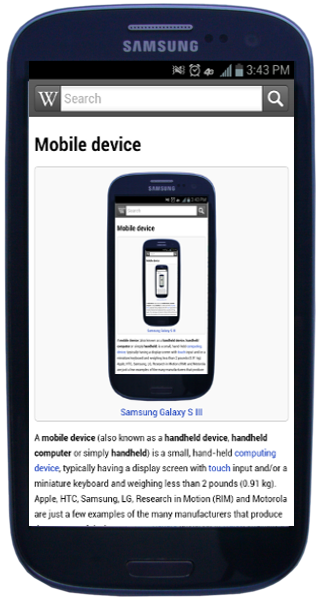
\includegraphics[height=0.25\textheight]{img/Samsung_Galaxy_S_III_Pebble_Blue_WikiWikipedia.png}
 \caption{Samsung Galaxy S3} \footnote{TEST}
\end{figure}

Da heutzutage der Mobilität eine große Bedeutung zusteht, steigt die Popularität des Mobilgerätes in der Bevölkerung und es wird von verschiedenen Personen zu verschieden Zwecken eingesetzt.  Mit der Entwicklung der Technologien kommen auch immer mehr universale Mobilgeräte auf den Markt, die zur Kommunikation, Navigation und Unterhaltung gleichzeitig genutzt werden können. 

% subsection mobile_ger_te (end)

\subsection{Einschränkungen in mobilen Kontexten} % (fold)
\label{sub:einschr_nkungen_in_mobilen_kontexten}
Bei der Entwicklung des Designs für die Mobilgeräte, stößt der Designer, laut Kuo-Ying Huang auf Probleme verschiedener Art, die die Hardware und die Software betreffen. 
Wie bereits erwähnt, gilt das für die Mobilgeräte das Prinzip "mobiler Kontext- immer und überall". Aus dem Grund spielt die Mobilität eine wichtige Rolle und zieht Einschränkungen bezüglich ihrer Größe und des Gewichts nach sich, was wiederum Hardware Einschränkungen zur Folge hat. Kuo-Ying Huang  unterscheidet zwischen drei Arten der Hardware-Einschränkungen: begrenzte Eingabemöglichkeiten, begrenzte Ausgabemöglichkeiten und Design für Mobilität.

% subsection einschr_nkungen_in_mobilen_kontexten (end)

\subsubsection{Begrenzte Eingabemöglichkeiten} % (fold)
\label{ssub:einschr_nkungen_in_mentalen_bereich}
Die meistverbreitete und grundlegende Eingabemöglichkeiten für Mobilegeräte auf dem Markt sind zurzeit: Tastatur, Touchscreen und Trackball.

Die Tastatur

Die Tastatur ist derzeit die Hauptmethode für Texteingabe.  Beim Drücken einer Taste, ermöglicht sie dem Benutzer die Eingabe von Symbolen, die Ausführung einer Aktion oder die Navigation der Menüpunkte. Leider ist sie in ihrer Standardgröße für Mobilgeräte nicht geeignet. Das Design der Tastatur kann zu einer der schwierigsten Aufgabe werden. Der Mangel an Platz des Mobilgerätes zwingt den Designer nach alternativen Lösungen zu suchen. Eine solche Lösung ist eine Telefontastatur mit Buchstaben. 

 \begin{figure}[h]
 \centering
 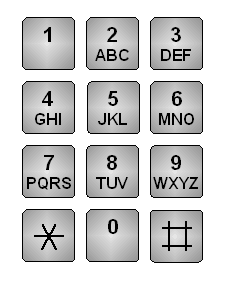
\includegraphics[height=0.25\textheight]{img/Tastatur_ITU-T-E161_4x3.png}
 \caption{Telefontastatur mit Buchstaben}
\end{figure}

Bei dieser Tastatur werden Buchstaben auf die zehn Zifferntasten verteilt. Man muss auf eine Taste bis zu viermal drücken, um einen Buchstaben zu treffen. Die Geschwindigkeit bei den kürzeren Texten (z.B. Kurznachrichten) war akzeptabel, aber bei den größeren Texten leider nicht.  Für Wearable Computing werden auch interessante Konzepte weiterentwickelt, wie z.B. die Akkordtastatur. Das ermöglicht dem Benutzer Symbole oder Befehle bei gleichzeitigen drücken der Tasten einzugeben. 

 \begin{figure}[h]
 \centering
 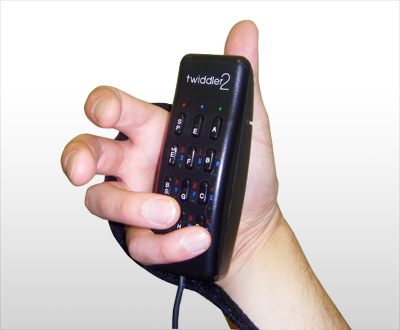
\includegraphics[height=0.25\textheight]{img/twiddler.jpg}
 \caption{Twiddler}
\end{figure}

Man könnte das mit dem Klavierspielen vergleichen. Vielzahl von Kombinationen aus einer kleinen Anzahl von Tasten, ermöglicht die Eingabe mit einer Hand, während die andere frei bleibt. Ein anderer Vorteil ist dadurch, dass die Größe dieser Tastatur geringer als die der Standarttastatur sein kann. Allerdings muss der Benutzer mehr Kombinationen erlernen, was als ein Nachteil gesehen werden kann.


Der Touchscreen

Der Touchscreen ist eine gute Alternative für die Tastatur und ermöglicht dem Nutzer tippen auf virtuelle Tastatur. Jedoch treten bei ihrer Benutzung auch Schwierigkeiten auf. Im Falle eines zu kleinen Bildschirmes sieht der Benutzer bei der Eingabe nicht die graphischen Elemente, das sogenannte " fat-finger syndrome".  Um dies zu vermeiden, gibt es auch verschiedene Konzepte.

 \begin{figure}[h]
 \centering
 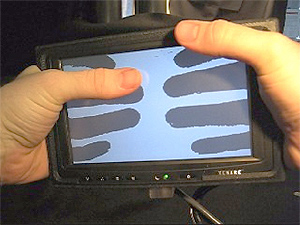
\includegraphics[height=0.25\textheight]{img/lucidtouch.jpg}
 \caption{The LucidTouch prototype}
\end{figure}

Eines davon ist LucidTouch (LucidTouch: A See-Through Mobile Device), das ist ein Eingabegerät, das es dem Benutzer ermöglicht, die Anwendungen zu steuern, indem er die Rückseite des Gerätes berührt, so dass die Vorderseite nicht von den Fingern verdeckt wird. Die Grundidee dabei ist, dem Benutzer die Illusion von Pseudo-Transparenz zu geben. LucidTouch unterstützt auch multi-toch input, was die 10 Fingereingabe ermöglicht. Auch Forschungen haben ergeben, dass viele Benutzer gerne mit der Rückseite ihres Geräts agieren.

Der Trackball

Der Trackball wird hauptsächlich zur Navigation eingesetzt, aber auch zur Ausführung von Aktionen, durch das Drücken darauf. Der Vorteil des Trackballs ist, dass man nur einen Finger benötigt, um horizontal und vertikal im Menu zu navigieren. Leider zur Texteingabe ist er schlecht geeignet.
Außer obengenannten Eingabemöglichkeiten gibt’s auch neue Techniken, wie z.B. Scpracheingabe. Dafür wird ein Mikrofon verwendet und spezielle Spracherkennungssoftware. Der Nutzer spricht in das Mikrofon und die gesprochenen Wörter und Sätze werden in Text oder Befehle konvertiert. Spracherkennung  gehört zu den schwierigsten Aufgaben der Signalverarbeitung. Gesprochene Sprache hat einen individuellen Charakter und verschiedene Menschen sprechen gleiche Sätze auf eigene Art und Weise. Ein Spracherkennungsprogramm sollte diese Äußerungen als gleich erkennen. Für Mobilgeräte gibt’s zwar schon einige gute Lösungen, wie z.b. Google Voice Search (http://www.google.com/mobile/voice-search/), Siri Personal Assistent (http://www.apple.com/ios/siri/) oder Vlingvo (vlingvo.com). Leider meistens davon benötigen eine Internetverbindung, was nicht immer möglich ist.



% subsubsection einschr_nkungen_in_mentalen_bereich (end)

\subsubsection{Begrenzte Ausgabemöglichkeiten} % (fold)
\label{ssub:einschr_nkungen_in_bedienung}

Der Bildschirm


Es existieren eine Menge verschiedener Ausgabemöglichkeiten für Mobilgeräte. Ein Bildschirm ist eine der grundlegendsten davon. Um die passende Bildschirmgröße zu finden, braucht man viel Zeit und Erfahrung. Ein großer Bildschirm ist gut, da er viel Platz bietet, allerdings auch Mobilitätsprobleme mit sich bringt. Außerdem verbraucht ein großer Bildschirm offensichtlich mehr Strom, als ein kleiner Bildschirm derselben Art, was zu öfteren Aufladungen führt. 

 \begin{figure}[h]
 \centering
 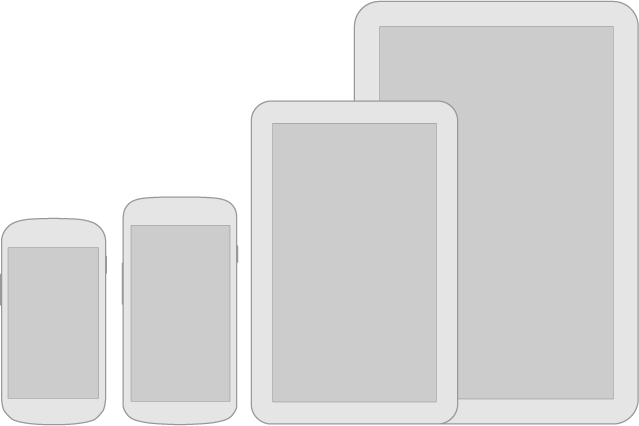
\includegraphics[height=0.25\textheight]{img/devices_displays_main.png}
 \caption{The LucidTouch prototype}
\end{figure}

Die Audio-Anlage und Vibration

Die Audio-Ausgabe ist eine weitere, oft verwendete Ausgabemöglichkeit für Mobilgeräte. Eine eingegangene Nachricht kann durch ein Ton-Singal in Verbindung mit grafischen Elementen und Text eine gute Interaktion zwischen Benutzer und Endgerät darstellen. In Mobilgeräten werden kleine und nicht leistungsstarke Lautsprecher eingesetzt. Das hat zur Folge, dass man beim großen Lärm eine wichtige Nachricht oder ein Ereignis verpassen kann. Eine gute Alternative ist eine Vibrationsfunktion. Im Mobilgerät wird ein kleiner Elektromotor eingebaut, der eine Welle antreibt. An der Welle hängt ein halber Zylinder und weil der Zylinder nur halb ist, hat er eine Unwucht, die bei schneller Drehung zu einer Vibration führt.


% subsubsection einschr_nkungen_in_bedienung (end)

\subsubsection{Design für Mobilität} % (fold)
\label{ssub:weiterf_hrung}

Da die Mobilgeräte immer und überall eingesetzt werden, entsteht das wichtigste Problem der Mobilität nämlich die Stromversorgung. Alle Hersteller wollen Akkus leistungsfähiger machen, leider sind sie nicht weit gekommen. Man kann mit einem Smartphone zurzeit nur ein Tag intensiv arbeiten. Es gibt zwar einige Verbesserungen bei den Akkus und sie konnten mithalten, aber durch die zusätzliche Technik, die größeren Bildschirme, die schnellen Netze und Prozessoren wird es wieder aufgezehrt.

% subsubsection weiterf_hrung (end)